\chapter{The Multivariate Normal Distribution}

Let's say that you are gathering statistics on a species of snail. You have found 89 snails.
Every snail has been weighted and had its shell measured. You have created a table like this:

\begin{tabular}{ c c }
Weight & Diameter \\
\hline
4.4769 grams & 2.2692 cm\\
5.4755 grams & 2.1973 cm\\
4.1183 grams & 2.52928 cm\\
... & ... \\
3.0522 grams & 1.7822 cm
\end{tabular}


You have been told that for any particular species of snail, the weight and shell diameter are typically normally distributed.
So, you compute the mean of each:

$$\bar{x} = \frac{\sum_{i=1}^{n} x_i}{n}$$

Your snails have a mean mass off 4.25 grams and a mean shell diameter of 2.35 centimeters.
Now you know where the center of each normal distribution will be.

To know how wide each normal distribution is, you need to compute the variance:

$$\sigma^2 = \frac{\sum_{i=1}^{n} (x_i - \bar{x})^2}{n}$$

(Reminder: The standard deviation is the square root of $\sigma^2$)

Plotting this data is shown in Figure~\ref{fig:pdfweight_diameter}.
\begin{figure}[htbp]
    \centering
    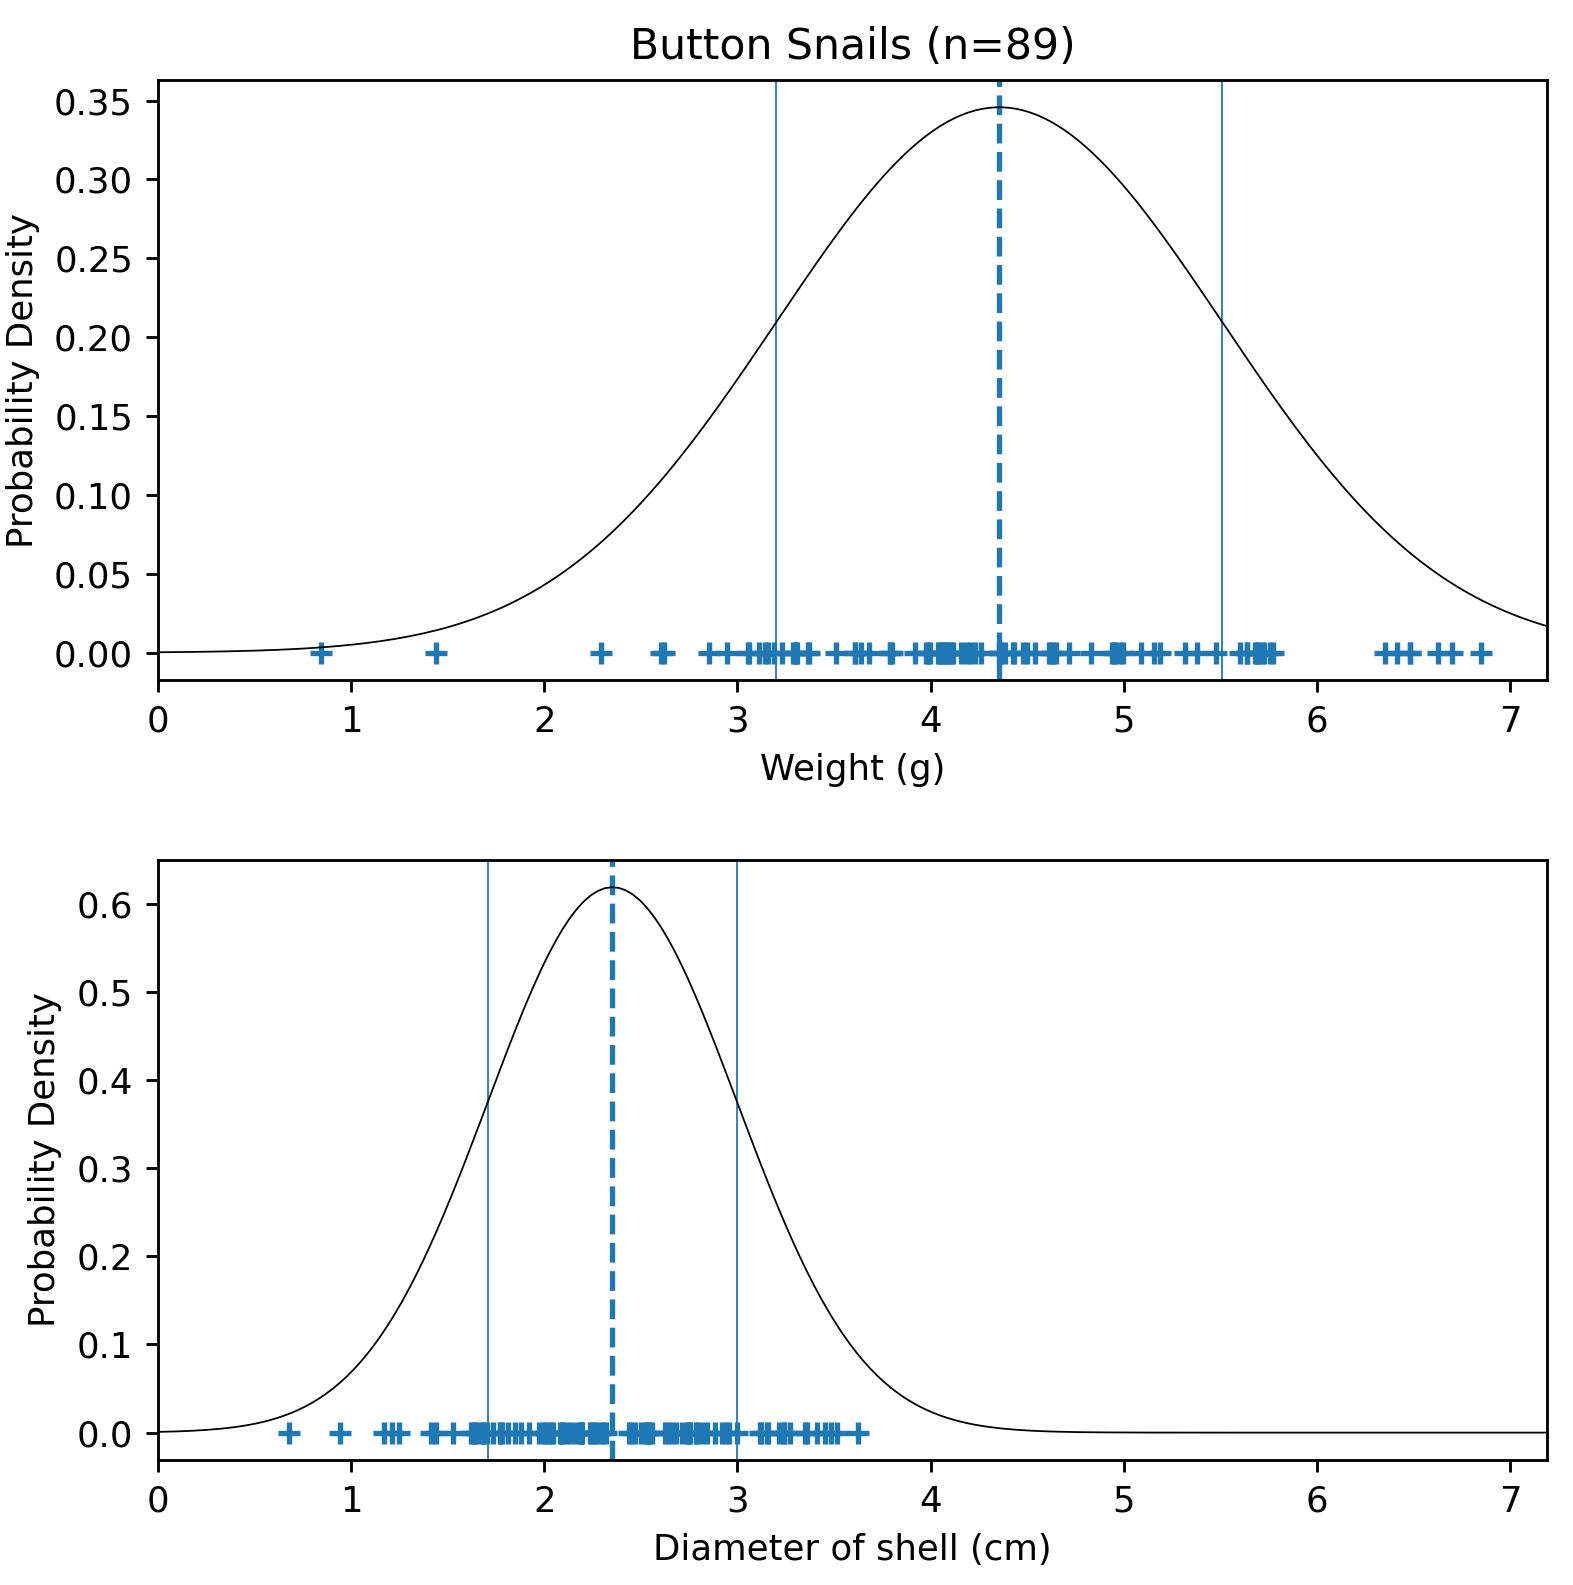
\includegraphics[width=0.55\textwidth]{separate.png}
    \caption{Probability density functions of weight and diameter.}
    \label{fig:pdfweight_diameter}
\end{figure}

Nice! However, then you think: "Hmm. Maybe the mass and the diameter of the shell are related. It seems like a heavy snail might tend to have a larger shell."  So, you make a scatter plot:

\begin{figure}[htbp]
    \centering
    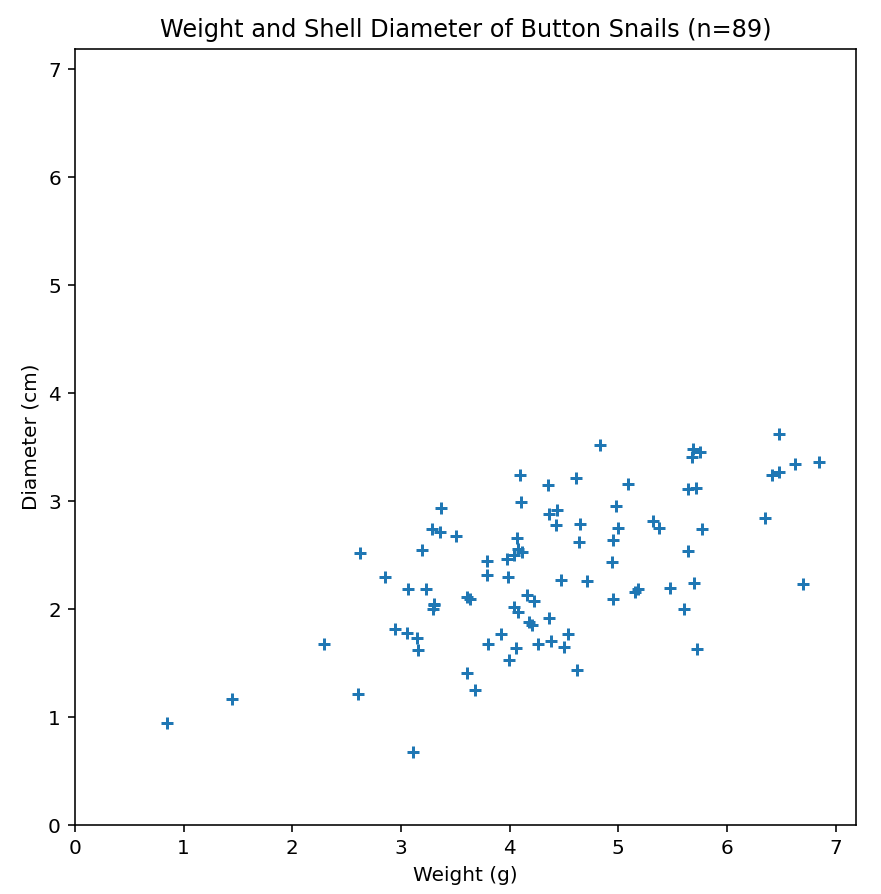
\includegraphics[width=0.55\textwidth]{scatter.png}
    \caption{A scatter plot with weight of the snail horizontally and diamter of the shell on the y-axis.}
    \label{fig:example}
\end{figure}

Sure enough, there is some correlation between the mass of the snail and the diameter of its shell.

There is a form of the normal distribution that can deal with multiple variables and their correlations.
This is known as the \newterm{multivariate normal} or the \newterm{Gaussian distribution}. \index{multivariate normal distribution} \index{Gaussian distribution}

In a multivariate normal distribution, the mean (often denoted $\boldsymbol\mu$) is a vector containing the mean of every variable.
For your snails, $\boldsymbol\mu = \begin{bmatrix} 4.25, 2.35 \end{bmatrix}$.

Just as in the single-variable normal distribution, measurements near the mean are what you are most likely to observe.
In a single-variable normal distribution, the standard deviation tells us how fast that likelihood falls off as we move away from the mean.
In multivariate normal distributions, we need something a little more expressive: a matrix.

\section{The Covariance Matrix}

We can think of the data as a list of vectors.
For example, if we have $n$ snails and $d$ properties that we have measured, we would get a list like this:

$$\begin{bmatrix}
x_{1,1} & x_{1,2} & ... & x_{1,d} \\
x_{2,1} & x_{2,2} & ... & x_{2,d} \\
... & ... & &... \\
x_{n,1} & x_{n,2} & ... & x_{b,d}\end{bmatrix}$$

Each row represents one snail. Each column represents one property.

Note that to make $\boldsymbol\mu$ (the mean vector), you just take the mean of each column of this data matrix. (For convenience, we will use $\boldsymbol\mu_i$ to refer to the mean of column $i$.)

We usually use $\mathbf{\Sigma}$ (the uppercase Greek sigma) to represent a covariance matrix. $\mathbf{\Sigma}$ is a $d \times d$ matrix.
The entries on the diagonal of $\mathbf{\Sigma}$ are just the variance of each property.
So, we can caluculate the entry at row $j$, column $j$ like this:

$$\mathbf{\Sigma}_{j,j} = \frac{\sum_{i=1}^{n}(x_{i,j} - \boldsymbol\mu_j)^2}{n}$$

(Yes, we are using $\mathbf{\Sigma}$ to represent both summation and the covariance matrix here.
It can be confusing, but you will be able to tell from context how it is being used.)

The other entries, $\Sigma_{j,k}$ where $j \neq k$, are the \newterm{covariance} between property $j$ and property $k$.
If the covariance is a positive number, property $j$ and property $k$ are correlated. For example, in your snails, weight and diameter have a positive covariance: If the snail is heavier than average, it tends to have a diameter that is larger than average.

If the covariance is a negative number, when property $j$ is greater than average, property $k$ tends to be less than average.
For example, the number of times a restaurant mops the floor in a week has a negative covariance with how much bacteria lives on the floor.

How do we compute the covariance?

$$\mathbf{\Sigma}_{j,k} = \frac{\sum_{i=1}^{n}(x_{i,j} - \boldsymbol\mu_j)(x_{i,k} - \boldsymbol\mu_k)}{n}$$

Note that $\mathbf{\Sigma}_{j,k} = \mathbf{\Sigma}_{k,j}$, so the matrix is symmetric.

\subsection{Computing Mean and Covariance in Python}

If you have a numpy array where each row represents one sample and each column represents one property, it is really easy to compute $\boldsymbol\mu$ and $\mathbf{\Sigma}$:

\begin{verbatim}
# Read in the data matrix, each row represents one snail
snails = ...

# Compute mu
mean_vector = snails.mean(axis=0)
print(f"Mean = {mean_vector}")

# Compute Sigma
covariance_matrix = np.cov(snails, rowvar=False)
print(f"Covariance = {covariance_matrix}")
\end{verbatim}

\section{Multivariate Normal Probability Density}

Now that we have good estimates of $\boldsymbol\mu$ and $\mathbf{\Sigma}$, how can we compute the probability density?

When you were working with just one variable, $x$, you computed the probability density using the mean $\mu$ and the variance $\sigma^2$ like this:

\begin{equation*}
p(x) = \frac{1}{\sqrt{2\pi\sigma^2}} e^{-\frac{(x - \mu)^2}{2\sigma^2}}
\end{equation*}

The probability density function of a $d$-dimensional
multivariate normal distribution with a mean of $\boldsymbol\mu$ and a covariance matrix of $\mathbf{\Sigma}$ is given by:

\begin{equation*}
p(\mathbf{x}) = \frac{1}{\sqrt{(2\pi)^d|\mathbf{\Sigma}|}}\exp\left(-\frac{1}{2}(\mathbf{x}-\boldsymbol\mu)^T\mathbf{\Sigma}^{-1}(\mathbf{x}-\boldsymbol\mu)\right)
\end{equation*}

If we draw lines to show where $\boldsymbol\mu$ is and contours to show lines of equal probability density, we get a plot shown in Figure~\ref{fig:contour_snail}.
\begin{figure}[htbp]
    \centering
    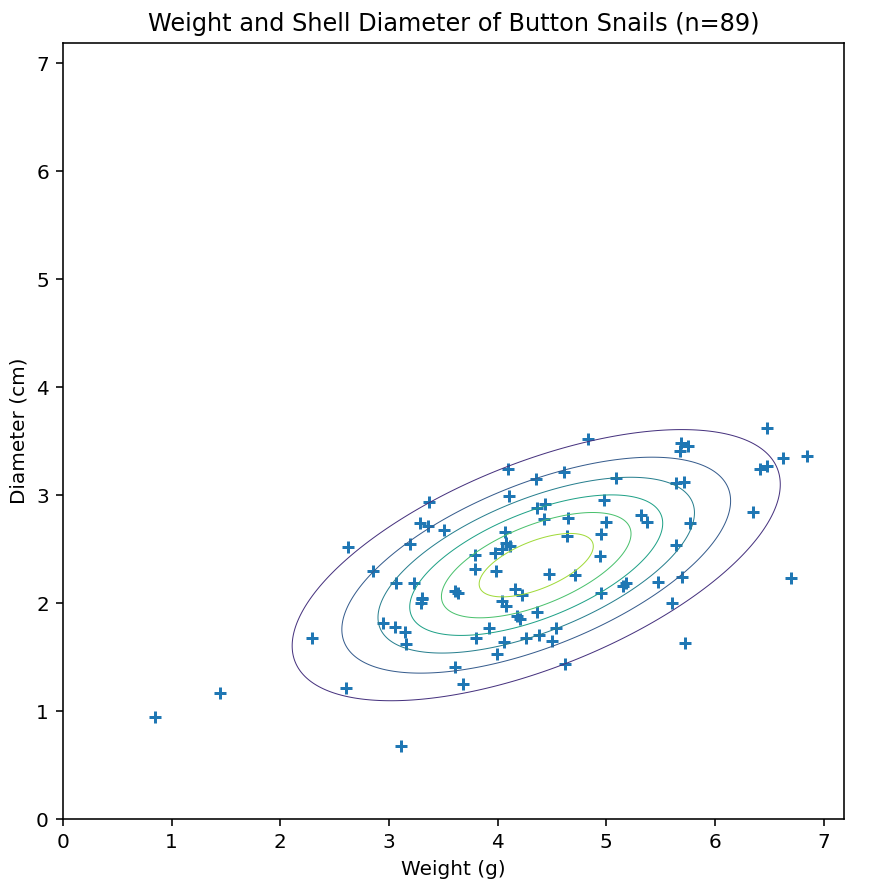
\includegraphics[width=0.55\textwidth]{contour.png}
    \caption{Contour plot of the snail data.}
    \label{fig:contour_snail}
\end{figure}

Or, we can do a 3D plot, as shown in Figure~\ref{fig:3d_snail}.
\begin{figure}[htbp]
    \centering
    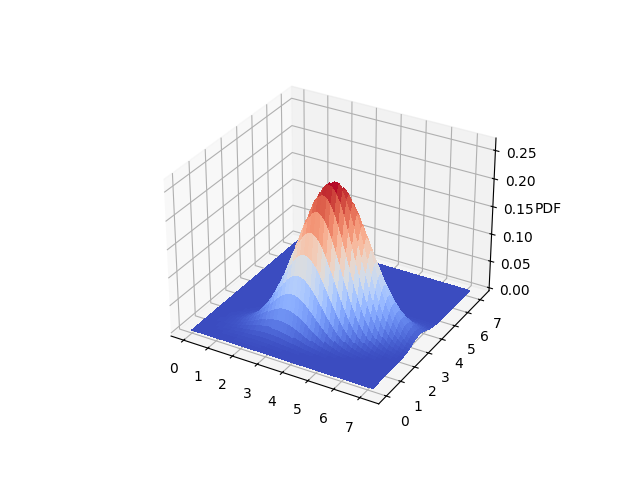
\includegraphics[width=0.55\textwidth]{3d.png}
    \caption{3D plot of the probability density function.}
    \label{fig:3d_snail}
\end{figure}

A probability density always integrates to 1.0, so the volume under the surface must be 1.0.

\subsection{Multivariate Normal Probability Density in Python}

The scipy library has a class that represents the multivariate normal. Here is how you could compute the probability density for a particular snail:

\begin{verbatim}
import numpy as np
from scipy.stats import multivariate_normal

...Compute mean_vector and covariance_matrix...

# Get the probability density at [3 grams, 2 cm]
x = np.array([3.0, 2.0])
pd = multivariate_normal.pdf(x, mean=mean_vector, cov=covariance_matrix)
print(f"The probability density at {x} is {pd}")
\end{verbatim}

Alternatively, maybe you would like to generate weights and diameters for a fictional population of 700 snails:

\begin{verbatim}
new_snails = multivariate_normal.rvs(mean=mean_vector, cov=covariance_matrix, size=700)
print(f"My fictional snails:\n{new_snails}")
\end{verbatim}
